%! suppress = Quote
%! suppress = MissingImport
%! suppress = MissingLabel
%! suppress = LineBreak

% CLI args https://tex.stackexchange.com/a/1501
\newif\ifhandout
\input{flags}

%! suppress = MissingLabel
%! suppress = DocumentclassNotInRoot
%! suppress = DiscouragedUseOfDef

% * Make friends tikz & colors
%   https://en.wikibooks.org/wiki/LaTeX/Colors
% * To enable vertical top alignment globally
%   https://tex.stackexchange.com/questions/9889/positioning-content-at-the-top-of-a-beamer-slide-by-default
% * Set handout from CLI
%   https://tex.stackexchange.com/a/1501
\ifhandout
\documentclass[usenames, dvipsnames, handout]{beamer} % https://tex.stackexchange.com/questions/224091/beamer-how-to-disable-pause-temporarily
\else
\documentclass[usenames, dvipsnames]{beamer}
\fi
% ------------------------------------------------

% Graphics
\usepackage{color}
\usepackage{tabularx}
\usepackage{tikz}
% https://tikz.dev/tikz-graphs
\usetikzlibrary{positioning, shapes.geometric, arrows, automata, graphs}
\tikzset{
    expr/.style={ellipse, draw=gray!60, fill=gray!5, very thick, minimum size=7mm, yshift=0.7cm},
    hexpr/.style={ellipse, draw=gray!60, fill=blue!15, very thick, minimum size=7mm, yshift=0.7cm},
    stmt/.style={rectangle, draw=gray!60, fill=gray!5, very thick, minimum size=5mm, yshift=0.7cm},
    decl/.style={rectangle, draw=blue!60, fill=gray!5, very thick, minimum size=5mm, yshift=0.7cm},
    hdecl/.style={rectangle, draw=blue!60, fill=blue!15, very thick, minimum size=5mm, yshift=0.7cm},
    subtree/.style={shape border rotate=90, isosceles triangle, draw=gray!60, fill=gray!5, very thick, minimum size=5mm, yshift=0.0cm},
}
\usepackage{blkarray}
\usepackage{graphicx}
\usepackage{forest} % https://tex.stackexchange.com/questions/198405/how-to-change-the-color-of-subtrees-in-tikz-qtree
% ------------------------------------------------

% Math
\usepackage{amsmath, amsfonts}
\usepackage{amssymb}
\usepackage{proof}
\usepackage{mathrsfs}
% Crossed-out symbols
% https://tex.stackexchange.com/questions/75525/how-to-write-crossed-out-math-in-latex
\usepackage[makeroom]{cancel}
\usepackage{mathtools}
% ------------------------------------------------

% Additional font sizes
% https://www.overleaf.com/learn/latex/Questions/How_do_I_adjust_the_font_size%3F
\usepackage{moresize}
% Additional colors
% https://www.overleaf.com/learn/latex/Using_colours_in_LaTeX
\usepackage{xcolor}
% Textual math symbols
\usepackage{textcomp}
% ------------------------------------------------

% Language
\usepackage[utf8] {inputenc}
\usepackage[T2A] {fontenc}
\usepackage[english, russian] {babel}
\usepackage{indentfirst, verbatim}
\usetikzlibrary{cd, babel}
% ------------------------------------------------

% Fonts: https://sites.math.washington.edu/~reu/docs/latex_symbols.pdf
\usepackage{stmaryrd}
\usepackage{cmbright}
\usepackage{wasysym}
\usepackage[weather]{ifsym} % https://tex.stackexchange.com/questions/100424/how-to-use-the-ifsym-package
% https://tex.stackexchange.com/questions/615300/pdflatex-builtin-glyph-names-is-empty
\pdfmapline{=dictsym DictSym <dictsym.pfb}
\pdfmapline{=pigpen <pigpen.pfa}
\usepackage{dictsym}
% ------------------------------------------------

% Code
% * Needs -shell-escape build flag
%   https://tex.stackexchange.com/questions/99475/how-to-invoke-latex-with-the-shell-escape-flag-in-texstudio-former-texmakerx
% * Set build directory
%   https://tex.stackexchange.com/questions/339931/latex-minted-package-using-custom-output-directory-build
\usepackage{minted}
\setminted{xleftmargin=\parindent, autogobble, escapeinside=\#\#}
% ------------------------------------------------

% Template
\usetheme{CambridgeUS}
\usecolortheme{dolphin}
% https://tex.stackexchange.com/questions/231439/beamer-how-to-make-font-larger-for-page-numbers
\setbeamerfont{headline}{size=\scriptsize}
\setbeamerfont{footline}{size=\scriptsize}
% Remove heddline
% https://tex.stackexchange.com/questions/33146/how-could-i-remove-a-header-in-a-beamer-presentation
%\setbeamertemplate{headline}{}
% Slide sizes
% https://tex.stackexchange.com/questions/56768/how-to-set-a-small-default-font-size-with-beamer
%\geometry{paperwidth=140mm,paperheight=105mm} % 4:3
\geometry{paperwidth=168mm,paperheight=105mm} % 16:10
% Remove navigation bar
% https://stackoverflow.com/questions/3210205/how-to-get-rid-of-navigation-bars-in-beamer
\beamertemplatenavigationsymbolsempty
% ------------------------------------------------

% Bullets
% https://9to5science.com/change-bullet-style-formatting-in-beamer
% https://tex.stackexchange.com/questions/185742/i-need-to-change-color-of-beamer-itemize-and-subitem-separately
\setbeamertemplate{itemize item}{\scriptsize\raise1.25pt\hbox{\donotcoloroutermaths$\blacktriangleright$}}
\setbeamertemplate{itemize subitem}{\scriptsize\raise1.5pt\hbox{\donotcoloroutermaths$\blacktriangleright$}}
\setbeamertemplate{itemize subsubitem}{\tiny\raise1.5pt\hbox{\donotcoloroutermaths$\blacktriangleright$}}
\setbeamertemplate{enumerate item}{\insertenumlabel.}
\setbeamertemplate{enumerate subitem}{\insertenumlabel.\insertsubenumlabel}
\setbeamertemplate{enumerate subsubitem}{\insertenumlabel.\insertsubenumlabel.\insertsubsubenumlabel}
% ------------------------------------------------

% Table of contents format
% https://tex.stackexchange.com/questions/642927/format-table-of-contents-in-beamer
\setbeamertemplate{section in toc}{%
        {\color{blue}\inserttocsectionnumber.}
    \inserttocsection\par%
}
\setbeamertemplate{subsection in toc}{%
        {\color{blue}\hspace{1em}\scriptsize\raise1.25pt\hbox{\donotcoloroutermaths$\blacktriangleright$}}
    \inserttocsubsection\par%
}
\setbeamertemplate{subsubsection in toc}{%
        {\color{blue}\hspace{2em}\tiny\raise1.25pt\hbox{\donotcoloroutermaths$\blacktriangleright$}}
    \inserttocsubsubsection\par%
}
% ------------------------------------------------

% Misc
\usepackage{multicol}
\usepackage{hyperref}
\usepackage{soul} % https://tex.stackexchange.com/questions/23711/strikethrough-text
% ------------------------------------------------

% Fix \pause for amsmath package envs (black black magic)
% https://tex.stackexchange.com/questions/16186/equation-numbering-problems-in-amsmath-environments-with-pause/75550#75550
% https://tex.stackexchange.com/questions/6348/problem-with-beamers-pause-in-alignments
%! suppress = Makeatletter
\makeatletter
\let\save@measuring@true\measuring@true
\def\measuring@true{%
    \save@measuring@true
    \def\beamer@sortzero##1{\beamer@ifnextcharospec{\beamer@sortzeroread{##1}}{}}%
    \def\beamer@sortzeroread##1<##2>{}%
    \def\beamer@finalnospec{}%
}
%! suppress = Makeatletter
\makeatother
% ------------------------------------------------

% Sections
\newcommand{\sectionplan}[1]{\section{#1}%
    \begin{frame}[noframenumbering]{Содержание}
        \tableofcontents[currentsection]
    \end{frame}
}
\newcommand{\subsectionplan}[1]{\subsection{#1}%
    \begin{frame}[noframenumbering]{Содержание}
        \tableofcontents[currentsubsection]
    \end{frame}
}
% ------------------------------------------------

% Footnotes
\renewcommand{\thefootnote}{\arabic{footnote}}
\renewcommand{\thempfootnote}{\arabic{mpfootnote}}
% https://tex.stackexchange.com/questions/28465/multiple-footnotes-at-one-point
\usepackage{fnpct}
% ------------------------------------------------

% Links
% Colors also links on slide foot.
%\hypersetup{
%    colorlinks=true,
%    citecolor=blue,
%    linkcolor=blue,
%    urlcolor=blue
%}
% ------------------------------------------------

% Appendix
% Slide numbers
% https://tex.stackexchange.com/questions/70448/dont-count-backup-slides
\usepackage{appendixnumberbeamer}
\newcommand{\backupbegin}{
    \newcounter{framenumbervorappendix}
    \setcounter{framenumbervorappendix}{\value{framenumber}}
}
\newcommand{\backupend}{
    \addtocounter{framenumbervorappendix}{-\value{framenumber}}
    \addtocounter{framenumber}{\value{framenumbervorappendix}}
}
% ------------------------------------------------

% Custom commands
% * Decor
\newcommand{\newtopic}[0]{$+$} % item: new topic on "in previous series"
\newcommand{\then}{$\Rightarrow$} % item: consequences
\newcommand{\pop}[0]{\SunCloud} %item:  general eduation
\newcommand{\popslide}[0]{(\pop)}
\newcommand{\advanced}[0]{$\varhexstar$} % item: advanced science
\newcommand{\advancedslide}[0]{(\advanced)}
\newcommand{\practical}[0]{\dstechnical} % item: practical programming notions
\newcommand{\practicalslide}[0]{(\practical)}
\newcommand{\todo}[0]{todo} % item: question
\newcommand{\answer}[0]{\Lightning} % item: answer to the previous question
\newcommand{\eg}[0]{e.g.} % item: example
\newcommand{\defi}[0]{$\Delta$} % item: definition on smth
\newcommand{\textdefi}[1]{\textbf{#1}}
\newcommand{\positive}{$+$} % item: pros
\newcommand{\negative}{{\color{red} $-$}} % item: cons
\newcommand%! suppress = EscapeHashOutsideCommand
\NB[1][0.3]{N\kern-#1em{B}} % default kern amount: -0.3em
\renewcommand{\emph}[1]{{\color{blue} \textit{#1}}}
\newcommand{\vocab}[1]{\textbf{#1}} % item: important new word
% * Lambda calculi
\newcommand{\comb}[1]{\mathbf{#1}} % defined combinator
\newcommand{\term}[1]{\mathbf{#1}} % predefined lambda-term reference
\newcommand{\termdef}{\coloneqq} % lamda term binding
\newcommand{\step}{\rightsquigarrow} % reduction step
\newcommand{\sstep}{\twoheadrightarrow} % multiple steps reduction
\newcommand{\ap}{~} % lambda-term application
\newcommand{\subst}[3]{\left[#2 \mapsto #3 \right] #1} % substitution
\newcommand{\eqbeta}{=_\beta} % beta equality
\newcommand{\eqeta}{=_\eta} % eta-equality
\newcommand{\eqt}{=} % tree-equality of terms
\newcommand{\tlist}[1]{\term{[}#1\term{]}} % list-term
% * Legacy
%\newcommand{\err}[0]{\textcolor{red}{ошибка}} % compilation error

% ------------------------------------------------

% Speaker notes
% https://tex.stackexchange.com/questions/114219/add-notes-to-latex-beamer
% https://tex.stackexchange.com/questions/35444/split-beamer-notes-across-multiple-notes-pages/35496#35496
%\setbeameroption{show notes on second screen=right} % enable speaker notes
%--------------------------------------

\author[]{Андрей Стоян, Илья Колегов, Дмитрий Халанский}
\institute[MSE ITMO]{MSE ITMO}


\title[5. Типы данных]{Практика 5. Типы данных}
\date{осень 2024}

\begin{document}

    \setcounter{framenumber}{-1}
    \maketitle

    \begin{frame}[fragile]{В предыдущих сериях}
        \begin{itemize}
            \item Структуры данных в чистом лямбда-исчислении
            \item Базовый синтаксис Haskell
            \item Базовые типы Haskell
            \item[\newtopic] Списки работа с ними
            \item[\newtopic] Алгебраические типы данных и сопоставление с образцом
        \end{itemize}
    \end{frame}

    \begin{frame}[noframenumbering]{Содержание}
        \tableofcontents
    \end{frame}

    \sectionplan{\texttt{data}}

    \begin{frame}[fragile]{Зачем структуры данных в Haskell}
        \begin{itemize}
            \item В $\lambda$-исчислении мы уже пользовались всеми необходимыми структурами данных
            \begin{itemize}
                \item Пары: $\term{pair}, \term{fst}, \term{snd}$
                \item Варианты: $\term{inl}, \term{inr}, \term{either}$
                \item Числа: $\term{zero}, \term{suc}, \term{natElim}$
                \item Списки: $\term{nil}, \term{cons}, \term{fold}$
            \end{itemize}
            \item Однако эти реализации не всегда годятся на практике\footnote{\color{blue} \url{https://reasonablypolymorphic.com/blog/review-codata/index.html}.}:
            \begin{itemize}
                \item Неэффективны для реального оборудования
                \item Слишком сложно типизируются
                \item Элиминация часто требует обхода всей структуры
            \end{itemize}
            \item Haskell имеет встроенную поддержку структур данных
            \begin{itemize}
                \item Эффективно представляются на уровне значений
                \item Просто и номинативно типизируются
            \end{itemize}
        \end{itemize}
    \end{frame}

    \begin{frame}[fragile]{Конструирование произведений}
        \vspace{-0.5em}
        \begin{block}{Декларация типа-произведения}
            \begin{minted}{Haskell}
                data CatT = CatD String Int
            \end{minted}
            \pause
            \begin{itemize}
                \item \texttt{CatT} --- имя типа (типовой константы)
                \item \texttt{CatD} --- конструктор данных: \mintinline{haskell}|CatD :: String -> Int -> CatT|
                \item \texttt{CatD} --- специальная функция, которая реализуется в самом языке
                \item Имена типов и конструкторов данных не пересекаются --- их можно называть одинаково
            \end{itemize}
        \end{block}
        \begin{block}{Конструирование}
            \begin{minted}{haskell}
                barsik :: CatT
                barsik = CatD "barsik" 42
            \end{minted}
        \end{block}
        \begin{block}{Количество значений}
            \begin{minted}{haskell}
                |CatT| = |String| * |Int|
            \end{minted}
        \end{block}
    \end{frame}

    \begin{frame}[fragile]{Конструирование сумм}
        \begin{block}{Декларация типа-суммы}
            \begin{minted}{haskell}
                data Pet = Cat CatT | Dog String Int | Parrot
            \end{minted}
            \pause
            \begin{itemize}
                \item Значение типа \texttt{Pet} можно конструировать несколькими различимыми способами
                \item \mintinline{haskell}|Cat :: CatT -> Pet|
                \item \mintinline{haskell}|Dog :: String -> Int -> Pet|
                \item \mintinline{haskell}|Parrot :: Pet|
            \end{itemize}
        \end{block}
        \begin{block}{Конструирование}
            \begin{minted}{haskell}
                petCat :: CatT -> Pet
                petCat cat = Cat cat
            \end{minted}
        \end{block}
        \begin{block}{Количество значений}
            \begin{minted}{haskell}
                |Pet| = |CatT| + |String| * |Int| + 1
            \end{minted}
        \end{block}
    \end{frame}

    \begin{frame}[fragile]{Элиминация алгебраических типов}
        \vspace{-0.5em}
        \begin{block}{Декларации}
            \begin{minted}{haskell}
                data CatT = CatD String Int
                data Pet = Cat CatT | Dog String Int | Parrot
            \end{minted}
        \end{block}
        \begin{block}{Паттерн-матчинг (сопоставление с образцом)}
            Элиминация структуры данных путём сопоставления её со способом конструирования.
            \begin{minted}{haskell}
                show :: Pet -> String
                show pet = case pet of #\pause#
                  Parrot -> "Parrot"
                  Dog name _ -> "Dog: " ++ name
                  Cat (CatD name _) -> "Cat: " ++ name
            \end{minted}
            \begin{itemize}
                \item Шаблоны могут быть вложенными для сложных структур данных
                \item[\defi] \vocab{Exhaustiveness} --- проверка компилятора, что все варианты конструирования рассматриваются при паттерн-матчинге (стараемся максимально использовать)
            \end{itemize}
        \end{block}
    \end{frame}

    \begin{frame}[fragile]{Задачки на питомцев}
        \begin{block}{Декларации}
            \begin{minted}{haskell}
                data CatT = CatD String Int
                data Pet = Cat CatT | Dog String Int | Parrot
            \end{minted}
        \end{block}
        \begin{itemize}
            \item[\todo] Дан питомец, добавьте префикс \mintinline{haskell}|"baron"| к его имени
            \item[\todo] По питомцу верните возраст
            \item[\answer] \pause
            \begin{minted}{haskell}
                baronify :: Pet -> Pet
                baronify pet = case pet of
                  Parrot -> Parrot
                  Dog name age -> Dog ("baron " ++ name) age
                  Cat (CatD name age) -> Cat (CatD ("baron " ++ name) age)
            \end{minted}
            \item[\answer] \pause
            \begin{minted}{haskell}
                data MaybeInt = Nothing | Just Int
                age :: Pet -> MaybeInt
                age pet = case pet of
                  Parrot -> Nothing
                  Dog _ age -> Just age
                  Cat (CatD _ age) -> Just age
            \end{minted}
        \end{itemize}
    \end{frame}

    \begin{frame}[fragile]{Задачки на рекурсивные типы}
        \begin{minted}{haskell}
            data Tree = Leaf Int | Branch Tree Int Tree
        \end{minted}
        \begin{itemize}
            \item[\todo] Вычислите глубину дерева
            \item[\todo] Вычислите сумму значений
            \item[\todo] Примените к каждому значению в дереве функцию
            \item[\answer] \pause
            \begin{minted}{haskell}
                height :: Tree -> Int
                height tree = case tree of
                  Leaf _ -> 1
                  Branch l _ r -> max (height l) (height r)
            \end{minted}
            \item[\answer] \pause
            \begin{minted}{haskell}
                incrementree :: (Int -> Int) -> Tree -> Tree
                incrementree f tree =
                  let rec = incrementree f in
                  case tree of
                    Leaf x -> Leaf (f x)
                    Branch l x r -> Branch (rec l) (f x) (rec r)
            \end{minted}
        \end{itemize}
    \end{frame}

    \sectionplan{Полиморфные \texttt{data}}

    \begin{frame}[fragile]{Полиморфные алгебраические типы}
        \begin{itemize}
            \item Тип значений в структуре данных определяется её пользователем
            \item Tип структуры данных зависит от типов значений
            \item[\todo] Абстрагируйте \mintinline{haskell}|Maybe| по типу содержимого
            \begin{minted}{haskell}
                data MaybeInt = Nothing | Just Int
                age :: Pet -> MaybeInt
            \end{minted}
            \item[\todo] Какие типы будут у конструкторов данных?
            \item[\todo] Закодируйте полиморфное дерево и функцию трансформации значений
            \item[\answer] \pause
            \begin{minted}{haskell}
                data Maybe a = Nothing | Just a
                age :: Pet -> Maybe Int
            \end{minted}
            \item[\answer] \pause
            \begin{minted}{haskell}
                Nothing :: Maybe a
                Just :: a -> Maybe a
            \end{minted}
            \item[\answer] \pause
            \begin{minted}{haskell}
                data Tree a = Leaf a | Branch (Tree a) a (Tree a)
                transform :: (a -> b) -> Tree a -> Tree b
                transform f (Leaf x) = Leaf (f x)
                transform f (Branch l x r) = Branch (transform f l) (f x) (transform f r)
            \end{minted}
        \end{itemize}
    \end{frame}

    \begin{frame}[fragile]{Система кайндов}
        \begin{itemize}
            \item Теперь у нас есть аппликация на уровне типов
            \item Нужна система типов над типами для контроля количества типовых аргументов
        \end{itemize}
        \begin{center}
            \begin{tikzpicture}
                \node [expr] (ap) {$@$ \mintinline{haskell}|:: *|};
                \node [expr] (maybe) [below left = of ap] {\mintinline{haskell}|Maybe :: * -> *|};
                \node [expr] (int) [below right = of ap] {\mintinline{haskell}|Int :: *|};
                \draw [->] (maybe) -- (ap);
                \draw [->] (int) -- (ap);
            \end{tikzpicture}
        \end{center}
        \begin{itemize}
            \item[\todo] \pause Определите кайнд конструктора типа
            \begin{minted}{haskell}
                data Free f a = Pure a | Free (f (Free f a))
            \end{minted}
            \item[\answer] \pause \mintinline{haskell}|Free :: (* -> *) -> * -> *|
        \end{itemize}
    \end{frame}

    \sectionplan{Списки}

    \begin{frame}[fragile]{\secname}
        \begin{itemize}
            \item Список --- это дерево с одной веткой
            \begin{minted}{haskell}
                data List a = Nil | Cons a (List a)
            \end{minted}
            \item Стандартный список использует операторы
            \begin{minted}{haskell}
                data [] a = [] | (:) a ([] a)
            \end{minted}
            \item Есть синтаксический сахар \mintinline{haskell}|[] a #$\equiv$# [a]| и \mintinline{haskell}|[1, 2, 3] #$\equiv$# 1 : 2 : 3 : []|
            \item[\todo] Реализуйте безопасную функцию взятия головы списка
            \item[\todo] Реализуйте функцию, дуплицирующую элементы с чётными номерами
            \item[\answer] \pause
            \begin{minted}{haskell}
                safeHead :: [a] -> Maybe a
                safeHead xs = case xs of [] -> Nothing; x:_ -> Just x
            \end{minted}
            \item[\answer] \pause
            \begin{minted}{haskell}
                dupEvens :: [a] -> [a]
                dupEvens = concat . map f . zip [0..] where
                  f (i, x) = if odd i then [x] else [x, x]
            \end{minted}
        \end{itemize}
    \end{frame}

    \begin{frame}[fragile]{Больше задачек на списки}
        \begin{itemize}
            \item[\todo] Реализуйте разворот списка
            \item[\todo] Реализуйте разворот списка эффективно
            \item[\answer] \pause
            \begin{minted}{haskell}
                reverse :: [a] -> [a]
                reverse [] = []
                reverse (x:xs) = reverse xs ++ [x]
            \end{minted}
            \item[\answer] \pause
            \begin{minted}{haskell}
                reverse xs = go [] xs
                  where
                    go :: [a] -> [a] -> [a]
                    go acc [] = acc
                    go acc (x:xs) = go (x:acc) xs
            \end{minted}
        \end{itemize}
    \end{frame}

    \begin{frame}[fragile]{Персистентные структуры данных}
        \begin{itemize}
            \item[\defi] \vocab{Эфемерный интерфейс} --- изменение структуры данных меняет саму эту структуру
            \begin{minted}{kotlin}
                xs.append(1)
                xs.append(2)
            \end{minted}
            \item[\defi] \vocab{Персистентный интерфейс} --- изменение порождает новую структуру, оставляя старую неизменной
            \begin{minted}{haskell}
                ys = 1 : xs
                zs = 2 : ys
            \end{minted}
            \item[\NB] В Haskell все структуры данных персистентные
        \end{itemize}
        \begin{center}
            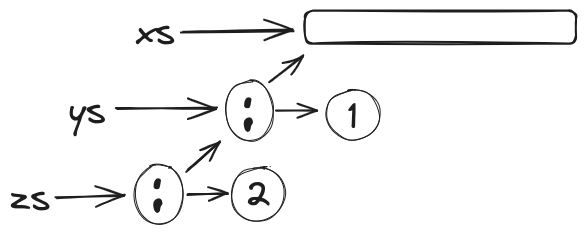
\includegraphics[width=0.7\textwidth]{figs/persistent-list}
        \end{center}
    \end{frame}

    \sectionplan{Всякое разное}

    \begin{frame}[fragile]{Записи (records)}
        \vspace{-0.5em}
        \begin{itemize}
            \item[\defi] Синтаксис для именования полей типов-произведений
            \item Синтаксис деклараций:
            \begin{minted}{haskell}
                data Cat = Cat { catName :: String, catMurlicity :: Int }
            \end{minted}
            \item Синтаксис создания (и, соответственно, паттерн-матчинга)
            \begin{minted}{haskell}
                cat = Cat { catName = "barsik", catMurlicity = 42 }
            \end{minted}
            \item Генерируются функции для доступа (применение --- \mintinline{haskell}|catName cat|):
            \begin{minted}{haskell}
                catName :: Cat -> String
                catMurlicity :: Cat -> Int
            \end{minted}
            \item Есть синтаксис для функционального обновления структуры:
            \begin{minted}{haskell}
                scratch cat = cat { catMurlicity = 1 + catMurlicity cat }
            \end{minted}
            \item[\practical] Использование с типами-суммы --- плохая практика (не тотальный код)
            \item[\practical] Засоряется глобальное пространство имён, поэтому используют префиксы имени типа
            \item[\practical] Для удобства работы существует множество расширений в компиляторе\footnote{\color{blue}\url{https://ghc.gitlab.haskell.org/ghc/doc/users_guide/exts/records.html}}
        \end{itemize}
    \end{frame}

    \begin{frame}[fragile]{Compile-time типовые обёртки: \texttt{newtype}}
        \vspace{-0.5em}
        \begin{itemize}
            \item Если у \mintinline{haskell}|data| один конструктор с одним параметром
            \item[\then] То выделять память под объект не обязательно --- храним сразу параметр
            \item[\defi] \mintinline{haskell}|newtype| --- более оптимальный вариант \mintinline{haskell}|data| для этого случая
            \item[\eg] На этапе компиляции --- разные типы, во время исполнения --- числа
            \begin{minted}{haskell}
                newtype ModuleId = ModuleId Int64
                newtype CourseId = CourseId Int64
            \end{minted}
            \item[\practical] Разные сущности предметной области должны иметь разные типы (по-хорошему)
            \begin{minted}{haskell}
                publish :: ModuleId -> CourseId -> Publisher Result
                main = ... publish courseId moduleId ... -- Compilation error
            \end{minted}
            \item[\practical] Обеспечение инвариантов значений программы:
            \begin{minted}{haskell}
                parseCourseId :: Int64 -> CourseId
                parseCourseId id | isValidCourseId id = CourseId id
                                 | otherwise = report error somehow
            \end{minted}
            \item[\practical] Возможен бесплатный переход между типами обёрток одного и того же
            \begin{minted}{haskell}
                intsToIds :: [Int64] -> [CourseId]
                intsToIds = #\framebox{\texttt{coerce}}#
            \end{minted}
        \end{itemize}
    \end{frame}

    \begin{frame}[fragile]{Очевидная тотальность \practicalslide}
        \begin{itemize}
            \item[\defi] \vocab{Тотальный код} --- никогда не расходится (зацикливания, исключения) --- утопия
            \begin{itemize}
                \item Завершаемость проверить нельзя (halting problem)
                \item Исключительные ситуации случаются (ошибки программиста, работа с IO)
            \end{itemize}
            \item Вместо этого используем ``\vocab{очевидную тотальность}''\footnote{Термин придуман и запатентован авторами презентации. По вопросам сотрудничества обращаться\ldots}
            \begin{itemize}
                \item Моделируем мир типами-суммы, используем exhaustive сопоставления с образцом
                \item Никогда не забываем базу рекурсии
                \item Делаем рекурсивный вызов на структурно меньших термах
            \end{itemize}
            \item На ошибке программиста --- всё же \href{https://en.wikipedia.org/wiki/Fail-fast}{\color{blue}fail fast}, чтобы не напортить ещё больше
            \item Выстраиваем чёткую границу с внешним миром (\underline{\color{blue} \href{https://lexi-lambda.github.io/blog/2019/11/05/parse-don-t-validate/}{Parse, don’t validate}})
            \begin{itemize}
                \item Данные парсим и преобразуем в структуры данных
                \item Активно используем \mintinline{haskell}|newtype| --- очень сильно недооценённая в промышленности концепция (но это пока --- Java inline classes, Rust tuple structs\ldots)
                \item В программе выполнение инвариантов уже гарантируется системой типов
            \end{itemize}
        \end{itemize}
    \end{frame}

    \begin{frame}[fragile]{Синонимы типов: \texttt{type}}
        \begin{itemize}
            \item Синонимы ничем не отличаются от соответствующих типов (взаимозаменимы в коде)
            \item Используются для придания типам доменно-специфичных имён:
            \begin{minted}{haskell}
                type Name = String
                showName :: Name -> String
                showName name = "Name: " ++ name
            \end{minted}
            \item А также для сокращения записи длинных типов
            \item Могут быть полиморфными (иметь типовой параметр)
            \begin{minted}{haskell}
                type State a = Map Name a
                State Int #$\equiv$# Map Name Int
            \end{minted}
        \end{itemize}
    \end{frame}

    \begin{frame}[fragile]{Полиморфные типы demystified или система $\lambda \omega$ \advancedslide\popslide}
        \begin{itemize}
            \item Подстановка типовых параметров в типы подозрительно напоминает подстановку термов в термы
            \begin{minted}{haskell}
                type Pair a b = forall c. (a -> b -> c) -> c
                Pair Int Char #$\equiv$# forall c. (Int -> Char -> c) -> c
            \end{minted}
            \item[\advanced] Это фактически она и есть (только для типов)!
            \begin{align*}
                &Pair : * \rightarrow * \rightarrow * \\
                &Pair = \lambda \tau^*~\sigma^*.~(\forall \gamma.~\tau\rightarrow\sigma\rightarrow\gamma) \\
                &pair : \forall \alpha~\beta.~\alpha \rightarrow \beta \rightarrow Pair~\alpha~\beta \\
                &pair = \Lambda \alpha^*~\beta^*.~\lambda x^\alpha~y^\beta.~(\Lambda \gamma^*.~\lambda f^{\alpha\rightarrow\beta\rightarrow\gamma}.~f~\gamma~x~y) \\
                &fst : \forall \alpha~\beta.~Pair~\alpha~\beta\rightarrow \alpha \\
                &fst = \Lambda \alpha^*~\beta^*.~\lambda p^{Pair~\alpha~\beta}.~p~\alpha~\mathbf{K}
            \end{align*}
        \end{itemize}
    \end{frame}

    \sectionplan{Алгебраические типы данных в других языках \popslide}

    \begin{frame}[fragile]{Типы-произведения в Си \popslide}
        \begin{block}{Декларация типа-произведения}
            \begin{minted}{C}
                struct CatTD {
                    string name;
                    int murlicity;
                };
            \end{minted}
            \begin{itemize}
                \item Имена типа и конструктора данных автоматически совпадают
            \end{itemize}
        \end{block}
        \begin{block}{Конструирование}
            \begin{minted}{C}
                CatTD createBarsik() {
                    return CatTD{"barsik", 42};
                }
            \end{minted}
        \end{block}
        \begin{block}{Элиминация}
            \begin{minted}{C}
                string getName(CatTD cat) {
                    return cat.name;
                }
            \end{minted}
        \end{block}
    \end{frame}

    \begin{frame}[fragile]{Типы-суммы в Си \popslide}
        \begin{minted}{c}
            struct Pet {
                enum { CAT; DOG; PARROT } tag;
                union {
                    struct { CatT catData } cat;
                    struct { Name name } dog;
                } value;
            };

            if (pet.tag == CAT) {
                printf("Cat: %s", pet.value.cat.catData.name);
            } else if (pet.tag == DOG) {
                printf("Dog: %s", pet.value.dog.name);
            } else if (pet.tag == PERROT) {
                printf("Perrot");
            } else {
                assert(false && "unreachable code"); // No exhaustiveness check
            }
        \end{minted}
    \end{frame}

    \begin{frame}[fragile]{Типы-суммы в ООП языках: пример на Python \popslide}
        \begin{minted}{python}
            class Pet: pass
            class Cat(Pet): cat: CatT
            class Dog(Pet): name: Name
            class Parrot(Pet): pass

            if isinstance(pet, Cat):
                print("Cat " + pet.cat.name)
            elif isinstance(pet, Dog):
                print("Dog " + pet.name)
            elif isinstance(pet, Parrot):
                print("Parrot")
            else:
                assert False, "unreachable code" // No exhaustiveness check
        \end{minted}
    \end{frame}

    \begin{frame}[fragile]{Типы-суммы в ООП языках: пример на Kotlin \popslide}
        \begin{itemize}
            \item Тюленезированные классы (wat?) заставляют определять всех наследников в пределах модуля
            \item Так у компилятора достаточно информации для проверки exhaustiveness
        \end{itemize}
        \vspace{1em}
        \begin{minted}{kotlin}
            sealed class Pet
            class Cat(val cat: CatT) : Pet
            class Dog(val name: Name) : Pet
            class Parrot : Pet

            when (pet) {
                is Cat -> print("Cat: " + pet.cat.name)
                is Dog -> print("Dog: " + pet.name)
                is Parrot -> print("Parrot")
            }
        \end{minted}
    \end{frame}

    \sectionplan{Материалы}

    \begin{frame}{Что посмотреть в транспорте}
        \begin{itemize}
            \item \href{https://lexi-lambda.github.io/blog/2019/11/05/parse-don-t-validate/}{\color{blue} \underline{Parse, don’t validate}}
            \item \href{https://youtu.be/qurG_J81_Cs?si=tINacE3c6ZF3CkvF}{\color{blue} Тагир Валеев — Pattern matching в Java и его воображаемые друзья}
        \end{itemize}
    \end{frame}

\end{document}
